\documentclass[12pt]{article}
\usepackage{amsmath}
\usepackage{graphicx}
\usepackage{hyperref}
\usepackage{listings}
\usepackage{color}

\title{Operating System Course Report - First Half of the Semester}
\author{B class}
\date{\today}

\begin{document}

\maketitle
\newpage

\tableofcontents
\newpage

\section{Introduction}
This report summarizes the topics covered during the first half of the Operating System course. It includes theoretical concepts, practical implementations, and assignments. The course focuses on the fundamentals of operating systems, including system architecture, process management, CPU scheduling, and deadlock handling.

\section{Course Overview}
\subsection{Objectives}
The main objectives of this course are:
\begin{itemize}
    \item To understand the basic components and architecture of a computer system.
    \item To learn process management, scheduling, and inter-process communication.
    \item To explore file systems, input/output management, and virtualization.
    \item To study the prevention and handling of deadlocks in operating systems.
\end{itemize}

\subsection{Course Structure}
The course is divided into two halves. This report focuses on the first half, which covers:
\begin{itemize}
    \item Basic Concepts and Components of Computer Systems
    \item System Performance and Metrics
    \item System Architecture of Computer Systems
    \item Process Description and Control
    \item Scheduling Algorithms
    \item Process Creation and Termination
    \item Introduction to Threads
    \item File Systems
    \item Input and Output Management
    \item Deadlock Introduction and Prevention
    \item User Interface Management
    \item Virtualization in Operating Systems
\end{itemize}

\section{Topics Covered}

\subsection{Basic Concepts and Components of Computer Systems}
This section explains the fundamental components that make up a computer system, including the CPU, memory, storage, and input/output devices.

\subsection{System Performance and Metrics}
This section introduces various system performance metrics used to measure the efficiency of a computer system, including throughput, response time, and utilization.

\subsection{System Architecture of Computer Systems}
Describes the architecture of modern computer systems, focusing on the interaction between hardware and the operating system.

\subsection{Process Description and Control}
Processes are a central concept in operating systems. This section covers:
\begin{itemize}
    \item Process states and state transitions
    \item Process control block (PCB)
    \item Context switching
\end{itemize}

\subsection{Scheduling Algorithms}
This section covers:
\begin{itemize}
    \item First-Come, First-Served (FCFS)
    \item Shortest Job Next (SJN)
    \item Round Robin (RR)
\end{itemize}
It explains how these algorithms are used to allocate CPU time to processes.

\subsection{Process Creation and Termination}
Details how processes are created and terminated by the operating system, including:
\begin{itemize}
    \item Process spawning
    \item Process termination conditions
\end{itemize}

\subsection{Introduction to Threads}
This section introduces the concept of threads and their relation to processes, covering:
\begin{itemize}
    \item Single-threaded vs. multi-threaded processes
    \item Benefits of multithreading
\end{itemize}

\subsection{File Systems}
File systems provide a way for the operating system to store, retrieve, and manage data. This section explains:
\begin{itemize}
    \item File system structure
    \item File access methods
    \item Directory management
\end{itemize}

\subsection{Input and Output Management}
Input and output management is key for handling the interaction between the system and external devices. This section includes:
\begin{itemize}
    \item Device drivers
    \item I/O scheduling
\end{itemize}

\subsection{Deadlock Introduction and Prevention}
Deadlock adalah kondisi dalam sistem komputasi di mana dua atau lebih proses tidak dapat melanjutkan eksekusi karena saling menunggu sumber daya yang sedang digunakan oleh proses lain. Deadlock terjadi ketika setiap proses dalam himpunan tersebut menunggu sumber daya yang dipegang oleh proses lain, sehingga menyebabkan lingkaran penantian yang tak berujung. Akibatnya, tidak ada proses yang dapat melanjutkan, dan sistem mengalami kebuntuan.

Model deadlock dapat dijelaskan menggunakan diagram graf alokasi sumber daya (\textit{Resource Allocation Graph} - RAG). Pada RAG, terdapat dua jenis simpul:

\begin{enumerate}
    \item \textbf{Proses}: Digambarkan sebagai lingkaran.
    \item \textbf{Sumber daya}: Digambarkan sebagai kotak atau persegi panjang.
\end{enumerate}

Setiap sumber daya mungkin memiliki beberapa unit yang dapat dialokasikan ke proses. Terdapat dua jenis edge (panah) dalam graf ini:

\begin{itemize}
    \item \textbf{Request edge (panah permintaan)}: Dari proses ke sumber daya, menunjukkan bahwa proses meminta sumber daya.
    \item \textbf{Assignment edge (panah alokasi)}: Dari sumber daya ke proses, menunjukkan bahwa sumber daya telah dialokasikan ke proses tersebut.
\end{itemize}

Contoh sederhana deadlock: Misalkan ada dua proses, P1 dan P2, serta dua sumber daya, R1 dan R2. Proses P1 memegang sumber daya R1 dan meminta R2, sementara P2 memegang R2 dan meminta R1. Maka terbentuk lingkaran penantian sebagai berikut:

\begin{enumerate}
    \item P1 $\rightarrow$ (request) R2
    \item P2 $\rightarrow$ (request) R1
    \item R1 $\rightarrow$ (assigned) P1
    \item R2 $\rightarrow$ (assigned) P2
\end{enumerate}

Karena kedua proses saling menunggu, sistem mengalami deadlock.

\begin{figure}[htbp]
    \centering
    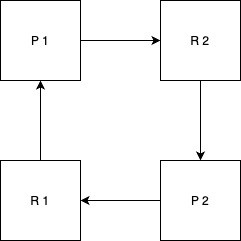
\includegraphics[width=0.5\linewidth]
    {asset/deadlockRAG.drawio.png}
    \caption{Contoh Diagram Deadlock dalam RAG}
    \label{fig:deadlock-RAG}
\end{figure}

Dalam diagram ini, P1 menunggu R2 dan P2 menunggu R1, sehingga keduanya tidak dapat melanjutkan eksekusi.

\subsubsection{Deadlock: Konsep Dasar, Contoh, dan Deteksi}

Deadlock adalah situasi di mana dua atau lebih proses mengalami kebuntuan karena saling menunggu sumber daya yang dipegang oleh proses lain. Deadlock sering terjadi pada sistem multiproses dan multithreading, di mana proses-proses berbagi sumber daya seperti memori, file, atau perangkat keras.

Sumber daya yang terlibat dalam deadlock dapat berupa:

\begin{itemize}
    \item \textbf{Sumber daya fisik}: seperti printer, port jaringan, CPU, atau memori.
    \item \textbf{Sumber daya logis}: seperti file, mutex, semafor, atau basis data.
\end{itemize}

Sistem operasi modern menghadapi risiko deadlock terutama pada sistem yang mendukung multitasking.

\subsubsection{Contoh Kasus Deadlock dalam Kehidupan Nyata}

Beberapa analogi yang menjelaskan deadlock secara visual:

\begin{itemize}
    \item \textbf{Contoh Jalan Raya}: Dua mobil berhadapan di jalan sempit, masing-masing menunggu yang lain mundur. Keduanya saling menunggu dan tidak ada yang dapat bergerak. Ini adalah situasi deadlock.
    \item \textbf{Contoh Restoran}: Seorang pelayan A memiliki kopi tetapi membutuhkan sendok dari pelayan B. Sementara itu, pelayan B memiliki sendok tetapi membutuhkan cangkir dari pelayan A. Keduanya tidak dapat menyelesaikan tugas karena saling menunggu.
\end{itemize}

\subsubsection{Deteksi Deadlock}

Pendekatan utama dalam menangani deadlock adalah deteksi deadlock, di mana sistem secara aktif memeriksa apakah telah terjadi deadlock dan mengambil langkah-langkah untuk menyelesaikannya.

Berikut beberapa metode untuk mendeteksi deadlock:

\paragraph{a. Penggunaan Resource Allocation Graph (RAG)}

RAG digunakan untuk memodelkan alokasi sumber daya ke proses. Jika ada siklus dalam graf ini, maka deadlock mungkin terjadi. Dalam RAG:

\begin{itemize}
    \item \textbf{Proses}: Digambarkan sebagai lingkaran.
    \item \textbf{Sumber daya}: Digambarkan sebagai kotak atau persegi panjang.
\end{itemize}

Jika ada siklus dalam graf ini, deadlock telah terjadi.

\paragraph{b. Algoritma Deteksi Deadlock pada Sumber Daya Tunggal}

Pada sistem di mana setiap sumber daya hanya memiliki satu instance, deteksi deadlock dilakukan dengan memeriksa apakah ada siklus dalam graf alokasi sumber daya. Jika siklus terdeteksi, maka deadlock terjadi.

\paragraph{c. Algoritma Deteksi Deadlock pada Sumber Daya Multipel}

Jika sebuah sistem memiliki beberapa instance dari jenis sumber daya yang sama, maka algoritma seperti \textit{Banker's Algorithm} dapat digunakan. Algoritma ini menilai apakah sistem dapat memenuhi semua permintaan sumber daya tanpa memasuki kondisi deadlock.

Dengan mengidentifikasi cara aman untuk mengalokasikan sumber daya, algoritma ini membantu mencegah terjadinya deadlock.

\paragraph{Referensi}
Ali A. \textit{151444239-Sistem-Operasi-Buku.pdf}. C.V.ANDI; 2005. p.212.

\begin{itemize}
    \item Deadlock conditions
    \item Deadlock prevention techniques
\end{itemize}

\subsection{User Interface Management}
This section discusses the role of the operating system in managing the user interface. Topics covered include:
\begin{itemize}
    \item Graphical User Interface (GUI)
    \item Command-Line Interface (CLI)
    \item Interaction between the user and the operating system
\end{itemize}

\subsection{Virtualization in Operating Systems}
Virtualization allows multiple operating systems to run concurrently on a single physical machine. This section explores:
\begin{itemize}
    \item Concept of virtualization
    \item Hypervisors and their types
    \item Benefits of virtualization in modern computing
\end{itemize}

\section{Assignments and Practical Work}
\subsection{Assignment 1: Process Scheduling}
Students were tasked with implementing various process scheduling algorithms (e.g., FCFS, SJN, and RR) and comparing their performance under different conditions.

\subsection{Assignment 2: Deadlock Handling}
In this assignment, students were asked to simulate different deadlock scenarios and explore various prevention methods.

\subsection{Assignment 3: Multithreading and Amdahl's Law}
This assignment involved designing a multithreading scenario to solve a computationally intensive problem. Students then applied **Amdahl's Law** to calculate the theoretical speedup of the program as the number of threads increased.

\subsection{Assignment 4: Simple Command-Line Interface (CLI) for User Interface Management}
Students were tasked with creating a simple **CLI** for user interface management. The CLI should support basic commands such as file manipulation (creating, listing, and deleting files), process management, and system status reporting.

\subsection{Assignment 5: File System Access}
In this assignment, students implemented file system access routines, including:
\begin{itemize}
    \item File creation and deletion
    \item Reading from and writing to files
    \item Navigating directories and managing file permissions
\end{itemize}

\section{Conclusion}
The first half of the course introduced core operating system concepts, including process management, scheduling, multithreading, and file system access. These topics provided a foundation for more advanced topics to be covered in the second half of the course.

\end{document}